\documentclass{article}
\usepackage{graphicx}
\usepackage{amsmath}
\usepackage{amsthm}
\usepackage{amssymb}
\usepackage{geometry}
\usepackage{twemojis}
\usepackage{subcaption}
\usepackage[style=numeric,bibstyle=numeric,backend=biber,natbib=true,maxbibnames=99,giveninits=true,uniquename=init]{biblatex}
\usepackage[utf8]{inputenc}
\usepackage{amsmath}
\usepackage{algorithm}
\usepackage{algpseudocode}
\usepackage{tikz}
\usetikzlibrary{positioning}

\addbibresource{../bibliography.bib}

% options: change 'markings' to 'entries'? include 'handwritten'?
\title{Fine-tuned optical character recognition for dental fossil markings}

\begin{document}

\tableofcontents

\section{Abstract}

Digitizing and uniformizing the structure of handwritten fossil catalogues exhibits a great 
potential for increasing the accuracy of paleontological data analysis by increasing sample sizes. 
Approximately 90, 000 of such samples reside in the archives of the National Museum of Kenya, and 
an ongoing effort is to store this data in a digital format for better accessibility.
A previous project utilized a commercial optical character recognition service for automated reading of these catalogues. This generalist
handwriting detection model lacked the ability to detect special characters used to denote tooth samples, and could not utilize prior knowledge 
of the vocabulary that is more likely to be present in the data, leading to loss of information and detection mistakes.

This thesis aims to build a specialist character recognition model to increase the accuracy of 
the bone or tooth type specifying column of the digitized data by fine-tuning a state-of-the-art optical 
character recognition model with few-shot transfer learning. This is performed by first finding most accurate
recognition models, variants of convolutional neural networks or vision transformers, and most successful 
transfer learning methods for adapting a model to a new character set. Then, the character 
recognition accuracy of combinations of these methods are benchmarked using handlabeled image segments from the 
fossil catalogues. The final aim of this work is to use the best-performing model 
to obtain an accurate reading of the catalogues of the National Museum of Kenya, and publish the final model to be used 
by the paleontological community for further digitization efforts.

Keywords: Optical character recognition, Transfer learning, Paleontological databases

\section{Introduction}


% use 'we' in intro

% outline of an introduction
% introduce the broad research area, why this is interesting. 1-2 paragraphs. context, anyone should be able to understand.
% first sentences: state the topic clearly
% broad research area: paleontology: data analysis on fossil finds
% dig fossil from the ground. identify:which bone,species,time. write this on a field slip, a slice of
% baking sheet like paper 
% analysis: take set of fossils, use methods for deducing eg climate, habitat, vegetation
% why this is interesting 
%     reactions of ecosystems to climate change
%     what ancient worlds were like 
%     how ancient humans lived
%     mass extinction events

The field of paleoecology conducts data analysis on fossil specimens.
Such analysis is quite literally started from the ground: after a fossil specimen has been found, it is 
carefully measured and identified: which bone and species the fragment is from, and how old it is. On site, such information is logged on field slips, small thin sheets of 
paper with a pre-printed form. The analysis has then been traditionally conducted by 
collecting such entries, sometimes collected in handwritten tabular catalogues, and running statistical 
tests on the sample set. With this analysis, facts from distant past, such as climate, habitats and 
vegetation can be deduced \cite{Faith_Lyman_2019}. Syntheses of such results consequently allow us to 
answer larger questions, such as how ecosystems reacted to climate changes, how mass extinction events 
came about, and what the living world could be like \cite{Žliobaitė2023}. Understandably, answering such 
questions has become ever more pressing.

% now we have a stack of baking sheets in a room in kenya.
% paleontologists form all over the world want to solve climate change, among other problems
% big data methods would explode what paleoecology can do
% so we need to put the baking sheets on the computer to do analysis on big data
% what is the topic of my work?
% the baking sheets contain weird characters that a normal reader cannot read.
% my topic is to read them

To find answers to large-scale problems, more sophisticated computational data analysis methods have come about,
relying on large datasets. Due to the infeasibility of collecting stacks of fields slips across sometimes multiple 
continents, specimens residing in archives of institutions have been converted to digital, public databases.
One such institution is the National Museum of Kenya, holding a large fraction of data collected from one 
of the most valuable fossil sites globally, the lake Turkana. The sheer amount of physical samples in the museum storage
makes keeping them safe a significant challenge, a risk to global heritage now recognized even by the White House and 
the United Kingdom government, as reported by the Wall Street Journal \cite{hotzMuseumOverflowingPrehistoric2024}.
 A project digitizing the handwritten catalogues hosted by the NMK was started by
using commercial optical character recognition software, combined with heuristical and machine learning approaches, 
resulting in satisfactory accuracy on conventional handwritten text. However, a large hurdle in the existing 
approach were the special characters used to denote which teeth each specimen contains. The aim of this work is 
to continue the project by digitizing these markings accurately.

% explanation of the specific problem
%given scanned images and data with bounding boxes of sentences and words where tooth denoting words are 
%badly read, how can tooth element recognition results be improved? Goal is to have both this is what the element 
%/ nature of specimen column says (eg example here) and what/which teeth are found in this specimen in standardized format
%(eg example here)
%the topic of my work is creating a tool that inputs cropped images from the sheets containing
%handwritten specifications of fossil bones and outputs what the text says

Specifically, this work uses as input data both scan images of the fossil slips and catalogues, and outputs from the Azure AI Vision software \cite{azurevision}. The existing outputs consist of sentence and word-level readings, along with bounding boxes defining 
the location of each word or sentence. The main research question is the following: 

How, given the input data, can the accuracy of the readings of the tooth markings be improved?

% brief review of standard solutions to this (or related) problem(s) and their limitation in this case (incl. reference key papers)
% TODO, once literature review is done


% outline of the new solution
% TODO, likely: tooth or not classifier -> trocr or tooth classifier -> output concatenation

% how the solution was evaluated, what were the results of this evaluations. scope and limitations
% TODO

% relevance for other work: why was this specific problem? how can this be concretely used?
% relevance of this work: KNM is able to have way more precise dental element markings
% to other catalogues: previous project + this a complete solution to digitizing the handwritten data 
% relevance of this work: any field that does:
% - ocr on unconventional characters
% - ocr where each character has a multivariate output (eg. this is an a. it is underlined could be letter and underlined /not underlined)

The direct impact of this work is an improved precision of the tooth element entries in the digitized 
fossil catalogues of the National Museum of Kenya, but the results are applicable to a wider domain of problems.
Intuitively, the results are directly applicable to other fossil archives using similar notation: only a fine-tuning of the 
models to the new archival data is necessary.
For other handwritten archives, the results presented can be used to improve recognition accuracy, especially in cases 
where the data contains characters other than latin letters or arabic numerals. Additionally, this work presents
a potential solution for when the target character set can be expressed with multivariate output data. This could, for 
instance, be handwriting with occasional underlinings, where the bivariate output could be the letter and a boolean variable for 
whether the character was underlined.

% organization
The rest of this thesis is organized as follows. First, the necessary background theory is 
presented. For deep neural networks, the following concepts are introduced:
the basic network structure, how training is conducted, basic building blocks of character-recognizing network architectures, performance-improving 
heuristics, and transfer learning. For paleoecology, the background covers 
foundational ecological laws followed by a brief introduction to methods used in
paleoenvironmental reconstruction, especially focusing on inferences from tooth data.
As the last background section, the composition of mammal teeth is presented. 
Second, related work is presented, both on
handwritten archive digitization and transfer learning with character-recognizer models.
Next, the experimental setup is introduced, covering dataset creation, labeling and data 
preprocessing, followed by base model and transfer learning method selection. After this, 
results of the experiments are presented and discussed. Finally, the work is concluded.

\section{Fundamentals on paleoecology}

\subsection{Basics on ecology}

\subsection{Paleoenvironmental reconstruction}

\subsection{Composition of mammal teeth}
\label{sect:mammal_teeth}

%Fossils occur when animal / plant remains are deposited in a sediment in a way that preserves 
%some part of its original form. Since teeth are the hardest material in animals, large fraction
%of found parts are teeth. Fossil finding is followed by identification to most specific taxon possible
%largely a technical skill (ch5), teeth are identified down to type and number, how manyeth the teeth are,
%counting from center to edge or other way round??
%specimen can be either one tooth or fragments of the jaw bone where there are multiple teeth (markings like M1-3)
% present teeth here

Since geological events tend to erode organic remains the faster the remain decomposes, the hardest materials in 
the corpse represent largest fractions of fossil datasets. These hard materials include shells, bones and especially teeth, and 
the last is prominent in fossil data analysis also due to the fact that they encode a diverse set of information on 
the livelihood of the organism \cite{Faith_Lyman_2019}. The identification of the fossil remain is done at the finest resolution possible,
preferring taxon information over just identifying the genus, for instance. Finest-resolution information 
derived from dental fossils are the taxon the tooth is from, and which tooth or teeth are found in the specimen.
This section presents the naming and indexing system for mammal teeth commonly used in paleontological datasets,
as described by Hillson \cite{Hillson_2005}, and some common shorthand versions present in the dataset digitized in this work.

% complete jaw-describing terminology
% the jaw bones
%lower jaw bones: mandibles, upper jaw: maxilla, premaxilla
% permanent and deciduous (D), nonpermanent "milk" teeth (laita vaan jos löytyy d-hampaita)
Specimens including more complete fragments of the jaw are described with terminology related 
to the jaw bones. All mammals share the same bone structure around the mouth: the lower jaw consists 
of two bones called \textit{mandibles}, joining in the middle, whereas the upper jaw consists of bones called 
\textit{maxilla} and \textit{premaxilla}, that also form large parts of the face.
A common trait across many mammals is also that the permanent teeth erupt in the 
youth of the animal, replacing the 'milk' or \textit{decidous} teeth. Shorthands commonly used for these 
terms are 'mand' for mandibles, and capital letter 'D' for the decidous teeth.

% types of mammal teeth
%four classes, front to back: three incisors (I), one canine (C), four premolars (P), three molars (M). top bottom left right. top/bottom noting upper jaw as superscript lower jaw as lower script, 
% purpose: incisor -> catching, canine -> stabbing / killing prey, molars are for chewing. premolars are bit like canines bit like molars, function varies lot
% between taxa including holding, cutting and chewing. also form and number of each present changes between taxa.
%sometimes lower jaw as line on top and upper jaw as line on bottom, sometimes both are used: upper script number with line on bottom. Line is "the other jaw"
%if there are less of a type of teeth eg two premolars, they might be no 1 and 2 or no 3 and 4
The tooth rows of mammals are classified to four classes; \textit{incisor}, \textit{canine}, \textit{premolar}
and \textit{molar} and indexed with a numbering system. Moving from the middle of the tooth row
towards the side, there are up to three 
incisors, used for catching food and denoted with the letter 'i'. Behind them is the canine tooth, used for cutting, and 
in case of predators, killing. This tooth is denoted with the letter 'c'. Behind the canine are up to four premolars, noted with 'p'. These 
teeth vary most between taxa in form and function with functions including cutting, holding and chewing food.
The teeth at the back of the row are called molars, 'm', and are primarily used for chewing. Molars, like the other tooth types, 
vary in number between taxa, and are at most three. The numbers are always increasing when moving back in the tooth row, but in
 the case of missing teeth in a taxon, the numbers do not necessarily start from one: instead, the number is chosen to 
have teeth with same numbers as alike each other as possible. Thus, a taxon with only two premolars might only have the teeth P3 and P4.


% directional terminology
% distal "far from center of body", proximal "close to center of body", mesial "close to mouth opening"
%right and left sides are always symmetrical, denoted simply L or R or Lt or Rt or left or right. left is left looking from the animal, not the observers perspective
Location of the tooth present in the fossil is described with directional terms specifying the side, jaw and the location on the jaw.
The most
intuitive are left and right describing the side, where one needs to note that each denotes the side from the viewpoint of the 
animal, not the observer. Mammal teeth are always symmetrical, thus every tooth always has the 
equivalent other-jaw counterpart. The distance of a tooth from the throat 
is described with the terms \textit{distal}, 'far from to the mouth' and \textit{mesial}, 'close to the mouth'. For skeletal bones, the term \textit{proximal}, 
'close to the center of the body' is often used instead of 'mesial'.
Short-form versions for these terms include capital 'L' or 'Lt' for left, capital 'R' or 'Rt' for right, 'dist.' 
for distal and 'prox' for proximal.
The jaw, upper or lower, has three dominant notation styles: one is to sub- or superscript tooth index numbers, other is to 
over- or underline tooth markings, and the last style, prominent in digital fossil data, is to set the tooth type letter to upper- or lowercase.
In each of these systems, a superscipt, underline, or capital letter denotes upper jaw, and conversely subscript, overline or lowercase letter denotes the lower jaw.
An illustration of the mammal tooth system is presented in Figure~\ref{image:mammal_teeth}. Terminology with corresponding shorthands are summarized in Table~\ref{table:terminology} and jaw notation styles in Table~\ref{table:jaw_notation}.

\begin{figure}[h]
    \centering
    \includegraphics*[scale=0.43]{../images/teeth_img_hillson_book.png}
    \caption{Mammal teeth composition, from Hillson \cite{Hillson_2005}.}
    \label{image:mammal_teeth}
\end{figure}

\begin{table}[ht]
    \centering
    \begin{tabular}{|l|l|l|}
        \hline
        \textbf{Term}       & \textbf{Meaning}                                   & \textbf{Shorthands}       \\ \hline
        Mandible            & Lower jaw bone                                     & mand.                     \\ %\hline
        Maxilla, Premaxilla & Upper jaw bones                                    &                           \\ %\hline
        Deciduous           & 'Milk teeth'                                       & D, d                      \\ %\hline
        Incisor             & Tooth type (front, middle)                         & I, i                      \\ 
        Canine              & Tooth type (between incisor and premolar)          & C, c                      \\ %\hline
        Premolar            & Tooth type (between canine and molar)              & P, p                      \\ %\hline
        Molar               & Tooth type (back of tooth row)                     & M, m                      \\ %\hline
        Distal              & Far from body center / mouth                       & dist.                     \\ %\hline
        Mesial              & Close to the mouth                                 &                           \\ %\hline
        Proximal            & Close to body center                               & prox.                     \\ \hline
    \end{tabular}
    \caption{Terminology related to mammal teeth with corresponding shorthands}
    \label{table:terminology}
\end{table}

\begin{table}[ht]
    \centering
    \begin{tabular}{|l|l|l|l|}
        \hline
        \textbf{Jaw}      & \textbf{Line Notation} & \textbf{Sub/Superscript Notation} & \textbf{Digital Notation} \\ \hline
        Upper         & $\text{M}^{\underline{1}}$      & m\textsuperscript{1}              & M1                        \\ 
        Lower         & $\text{M}_{\overline{1}}$ & m\textsubscript{1}                & m1                        \\ \hline
    \end{tabular}
    \caption{Dental marking styles, Example: first molar. Line notation displayed in common style combining sub- and superscripts.}
    \label{table:jaw_notation}
\end{table}


% summary of chapter

\section{Deep Neural Networks for Optical Character Recognition}

% introduction to chapter
% point of this section: present relevant deep learning theory
% running example: reading characters from images (optical character recognition, OCR)

This chapter presents relevant background on deep neural networks (DNN), also known 
in literature as artificial neural networks (ANN) or, for historical reasons, multilayer perceptrons (MLP).
The aspects presented are constrained to those relevant to the problem at hand, optical character recognition (OCR),
that is also used as a running example.

\subsection{Deep Neural Networks}

% what is a neural net
% yes what is a neural network? function?
% weights in layers: floating point numbers, grouped in groups 
% activations: connections between weights, nonlinear scalar to scalar functions 

Neural networks are multivariate functions that share a specific form.
The function parameters, usually floating-point numbers, are called weights and are organized in groups called layers.
The first layer is called the input layer, after which there are multiple hidden layers, followed by the output layer.
Weights of adjacent layers are combined by activation functions, that are constrained to nonlinear functions with 
scalar inputs and outputs~\cite{princebook}. Simplest of the activation functions is the rectified
linear unit ReLU, shown in Equation~\ref{eq:relu}. A neural network is usually visualized with a graph structure, as seen in Figure~\ref{image:neuralnet}, where a node represents a 
weight, and an edge denotes that the value on the first layer is used to compute the value on the latter.

\begin{align}
    \text{ReLU}(x) = \max(0, x)
    \label{eq:relu}
\end{align}

\begin{figure}[h]
    \centering
    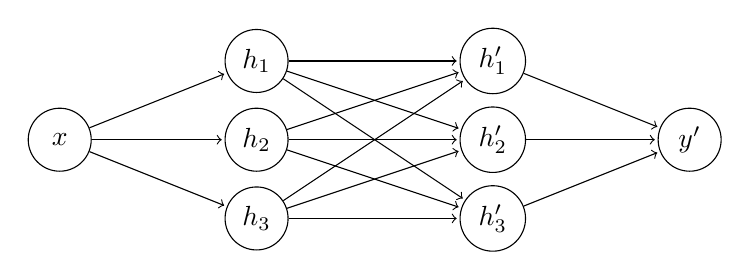
\begin{tikzpicture}[->, shorten >=1pt, auto, node distance=1.5cm, main node/.style={circle, draw, minimum size=0.8cm}]

        \node[main node] (x) {$x$};
        \node[main node] (h1) [right of=x, xshift=1cm, yshift=1cm] {$h_1$};
        \node[main node] (h2) [right of=x, xshift=1cm] {$h_2$};
        \node[main node] (h3) [right of=x, xshift=1cm, yshift=-1cm] {$h_3$};

        \node[main node] (h1') [right of=h1, xshift=1.5cm] {$h_1'$};
        \node[main node] (h2') [right of=h2, xshift=1.5cm] {$h_2'$};
        \node[main node] (h3') [right of=h3, xshift=1.5cm] {$h_3'$};

        \node[main node] (y) [right of=h2', xshift=1cm] {$y'$};

        % Edges
        \foreach \i in {1, 2, 3} {
            \draw (x) -- (h\i);
            \draw (h\i) -- (h1');
            \draw (h\i) -- (h2');
            \draw (h\i) -- (h3');
        }

        \foreach \i in {1, 2, 3} {
            \draw (h\i') -- (y);
        }
    \end{tikzpicture}
\caption{Visualization of a neural network with scalar input and output, and two fully connected layers, redrawn after~\cite{princebook}.}
\label{image:neuralnet}
\end{figure}

% - feed forward
% network computes output from input with the feed forward.
% you have an input, bunch of numbers
% then, you compute a linear combination and pass that through an activation function 

The computation of an output based on an input in the network is called the 
feed-forward, as the computation runs forward layer by layer through the 
network. The process starts from the input layer, which is simply the input 
organized as a vector. Each intermediate value on the first hidden layer, noted $h_d$ below,
is computed by taking a linear combination of the layer weight vector $\mathbf{\theta}$ and 
the input vector $\mathbf{x}$ of size $N$, adding the 
bias term $\theta_0$, and passing the result through the activation function $a$:

\begin{align}
    h_d = a\left[ \theta_{0} + \sum_{i=1}^{N}\theta_{di}x_{i} \right]
\label{eq:fc_layer}
\end{align}

% mean that this computation is done in a different manner (conv, transformer)
Different types of layers, such as convolutional or transformer layers 
denote that this single-layer computation process is performed differently from 
the standard form. When many layer types are present, layers using the computation
in Equation~\ref{eq:fc_layer} are called fully connected or dense layers.

% a is any nonlinear funtion, simplest is the rectified linear unit relu, x=x if x>0, x=0 if x<0.
% hidden units are taken as inputs to next layer and next and next. thetas = weights
% largest, deepest: hundreds of layers, hundreds of millions of weights 
% then last hidden unit output it the output of the network. tadaa.
The computation proceeds from the first hidden layer in a similar manner: 
the next layer values, also called activations, are computed using the weights of 
the layer and the previous layer activations with Equation~\ref{eq:fc_layer}.
The activations of the output layer is the output of the network.
More complex networks are generally constructed by increasing the network size to up to 
hundreds of layers with hundreds of millions of parameters, and by using
different types of layers.

% - universal function approximator
% the theory of the universal approximation capacity: this algebraic construct, 
% given correct weights, activation functions and structure, could approximate 
% any mapping from input to output. note: input/output dimension can be anything
The universal function approximator theorem states that functions belonging to the 
neural network family are capable of approximating any mapping from any type or shape of input
to any output with arbitrary precision \cite{princebook}. Naturally, due to high computational 
costs of finding the optimal weights and the large search space of possible networks, 
this theoretical optimum is rarely reached.

% examples from ocr relevant in this case
% input is always image ie 2d matrix if grayscale or 3d tensor if rgb image.
Examples of input-output mappings relevant in this work are the following, 
ordered from simplest to most complex: tooth type classification, constrained multilabel classification, 
and sequence-to-sequence learning. The problem of tooth type classification takes in an input image of a dental marking,
% this figure: see first all background & what samples are needed from tooth data...
such as input in Figure TODO a, and decides which tooth the image denotes.
As mammals have up to eleven teeth on each side of two jaws, the classes would be 
these 44 teeth, such as 'rm1', 'lP4' or 'li2', using the computational notation presented in
Section~\ref{sect:mammal_teeth}. The network would output a 44-element discrete probability distribution 
obtained by using the softmax function (Equation~\ref{eq:softmax}), that takes as input the last layer output
values and returns an output layer vector of the same length but with values between zero and one and summing to one, 
thus a valid probability distribution.
Here, like in other classification tasks, each value notes the probability that the image contains 
the tooth this value is chosen to represent. The final output would then be the largest probability
found in this vector.

\begin{align}
    \text{softmax}_k[\mathbf{z}] = \frac{\exp[z_k]}{\sum_{k'=1}^{K} \exp[z_{k'}]},
    \label{eq:softmax}
\end{align}

% multilabel classification problem:
% image of tooth sample. output: first MIPC, second if it is upper or lower jaw
% output can be two arrays, one like before, other a 0-1 probability for upper jaw. upper if this > 0.5 
A better approach that could encode the fact that all teeth of same type share a similar input feature
, a letter in the image, could be formulating the problem as a multilabel
problem \cite{multilabel_classification}: the output would be three of the aforementioned 
probability vectors, one with four elements representing 'M', 'P', 'C' or 'I', one with four elements 
for tooth indices, and two two-element vectors for left-right and upper-lower jaw. As this 
formulation lacks the notion that some tooth-type pairs never exist, such as the 4th canine,
this is a case of constrained multiclass classification, where some label pairs are marked 
as impossible combinations.

% present sequence to sequence learning:
% more complex case: image of sentence
% output: text on image, variable length. here output layer is a more complex 
% structure of probabilities for each position in the result sequence.
Generalizing the mapping problem further, one could also input a variable-length image 
of the entire dental marking comprising of multiple words, and outputting the text on this image.
Due to the variable output length, a special technique called sequence-to-sequence learning 
is employed \cite{sutskever2014sequence}. This encodes the fixed-length output layer to variable-length 
output text. Even though all of the problems presented in this section recognize characters, 
generally the term 'optical character recognition' is used for this type of mapping. Models
for solving these problems accurately are very large, for instance the Microsoft TrOCR has approximately 
500,000 parameters \cite{li2021trocr}.

Finding the best network weights for any of these types of input/output mapping problems, training 
a network, is conducted with the same process.
The general recipe for training a neural network is the subject of the next section.

\subsection{Training neural networks}

% u have encoded the structure, starting weights. data, input/output pairs.
% training = process that adjusts weights so that network becomes a good 
% approximator
After one has defined a neural network structure, initialized the weights of the network 
to some initial values and obtained a sufficiently large set of input-output pairs from the problem at hand,
one can start training the network. Training is an iterative process where inputs are used to 
predict the output, which is then compared to the ground truth. A more detailed account of these iterations
is presented next.

% 1. take part of data as training data
% 3 divide to batches, common batch sizes are exponents of 2, 2-32 usually 
At the start of training, a small fraction, commonly 10-20\%, is reserved as test data. Cross-validation is 
generally not used with neural networks due to the computational cost of the training process (ref?). The remainder, 
the training set, is divided into batches, sizes of which are commonly exponents of 2.

% 4. pass a batch through the network. get output 
% 5. pass output and correct to loss function: map from output, correct to scalar,
% 0 is good, large value bad.
% 6. Compute loss function gradient with respect to network weights using automatic differentiation.
% algorithm to get this in code is called backpropagation because it moves backward in the network
In an iteration of neural network training, a batch, stacked in a tensor of dimension one larger than the dataset, 
is passed through the network: outputs are computed based on the training inputs with the feed forward process.
After this, a loss function is used to evaluate the quality of the output: the loss function maps the network output and 
the correct output recorded in the training batch and outputs a scalar value, small value denoting a good 
match. Loss functions used in optical character recognition are presented in Section~\ref{sect:loss_funcs}.
After this follows a step called backpropagation: the gradient of the loss function with respect 
to the neural network weights is computed. The algorithm used in this computation is called automatic differentiation,
and is able to compute gradients with equal computational complexity as the feed forward by utilizing 
a variant of the chain rule and by proceeding backward in the network \cite{princebook}.

% 7. gradient informs how to adjust weights so that loss should decrease. 
% adjust weights in this direction by preset amount called learning rate. Optimizers
% are algorithms that determine the specifics of "moving in the direction of decreasing loss"
% most common stochastic gradient descent (inserts randomness to movement) and 
% adam (uses previous iteration movements known as momentum in process to make movements more smooth)
Once the gradient is computed, the next step is to choose how to adjust the network weights 
based on the gradient information. The simplest approach is, given a predefined step size 
known as the learning rate, to adjust the weights by the magnitude of the learning rate 
in the direction of fastest decreasing gradient, a heuristic called gradient descent. Different options for this approach 
are generally called optimizers and finding a suitable one is a fairly complex problem.
Other known optimizers are stochastic gradient descent (SGD), that inserts randomness 
to the weight-adjusting steps, and Adam (Adaptive Moment Estimation), that 
uses moments or gradients obtained in previous steps to add smoothness to the 
movement trajectory \cite{princebook}. After a weight-adjusting step is completed 
with the optimizer, the training iteration is completed.

% 8. run  batches until out of data  = epoch. run many epochs, stop according to 
% stopping condition that is known to be a state when the network weights are good.
% goal: reach global minimum of loss function, difficult! would be perfect approximation
The training process consists of repeatedly performing the aforementioned training 
iterations. Once the all batches of the whole dataset are used for training,
a training step known as epoch is completed. An usual a training process 
completes dozens or hundreds of epochs. The training is terminated once a predefined 
stopping condition, such as a number of epochs or a sufficiently small gradient 
magnitude, is met. The goal of the training process is to find the global minimum of the loss 
function with respect to the network weights, as this setting would correspond to 
the optimal approximation of the input-output mapping. Like with optimizers, 
determining optimal stopping conditions is a difficult problem area within neural network optimization.

% 8. test on unseen test data to see generalization performance
After the training is completed, the test dataset laid to the side at the start of 
training is used to evaluate the predictive power of the network on unseen data, 
also known as generalization performance. Metrics for measuring the accuracy 
of a readily-trained model are presented in Section~\ref{sect:eval_metrics}.
At this point the model should be considered 'frozen', as adjusting it would 
optimize the model to the small test set, not the general problem. This pitfall is 
known as 'data leakage' \cite{engbook}.

% lots of details on this process, rest is about that
% summarize: pseudocode of neural network training process
As is evident from the generality of the previous description, there are numerous 
specific aspects to consider when designing highly accurate neural networks. The 
rest of this chapter presents a snapshot of this problem area, focusing on those 
relevant to our problem of recognizing handwritten characters, and the rest of the 
work will experiment with parts of these aspects. A summarizing pseudocode of the 
neural network training process with gradient descent is presented in Algorithm~\ref{alg:net_training}.

\begin{algorithm}
    \caption{Neural Network Training}
    \begin{algorithmic}[1]
        \State \textbf{Input:} training\_data, epochs, learning\_rate
        \State Initialize weights $W$ randomly
        \State Initialize biases $b$ randomly
        
        \For{epoch = 1 to epochs}
            \For{each (input, target) in training\_data}
                \State $output \gets \text{ForwardPropagation}(input, W, b)$
                \State $loss \gets \text{CalculateLoss}(output, target)$
                \State $(gradients\_W, gradients\_b) \gets \text{BackwardPropagation}(input, output, target, W, b)$
                \State $W \gets W - learning\_rate \times gradients\_W$
                \State $b \gets b - learning\_rate \times gradients\_b$
            \EndFor
            \State Print("Epoch:", epoch, "Loss:", loss)
        \EndFor
        
        \State \textbf{Output:} $W, b$  \Comment{Trained weights and biases}
    \end{algorithmic}
    \label{alg:net_training}
\end{algorithm}

\subsubsection{Loss functions}
\label{sect:loss_funcs}

% more specific: how do you map output and label to scalar value describing how good the output was?
% ocr point of view
% Loss function is a function from model predictions and ground truth labels that describes with a single 
% scalar value how good the match was, low number describing a good match \cite{princebook}.
Loss functions are needed within the neural network training process to evaluate the model output 
quality in each training iteration. These functions map two equally shaped inputs, the predicted 
and true labels, to a scalar value describing match quality, a low value representing a good match \cite{princebook}. 
Thus, for instance, the simple function $f: x,y \rightarrow |x-y|$  would qualify as a loss function.
The most commonly used loss functions in optical character recognition are cross-entropy for 
character classification and the CTC loss for sequence learning.

% These functions are constructed to be equivalent with maximum likelihood solution, think the model would 
% output a conditional distribution of outputs, p(y|x).
% each ground truth label in the training set should have a high probability in this distribution. Product of all 
% these probabilities is called likelihood.
% Loss functions are derived so that parameters bringing loss to zero is equivalent to the parameters with maximum likelihood.
% Derivations are out of scope.
Loss functions are constructed usin maximum likelihood estimation. When one frames the neural network as outputting 
a conditional distribution $P(y|X)$, $y$ being the network output and $X$ the input, each correct label in the 
training set should have a high probability in this distribution. The likelihood is obtained by taking the product of 
all ground truth label occurence probabilities, and the training goal becomes maximizing this value. Loss functions are derived 
from the maximum likelihood formalization, so that the network parametrization associated with zero loss is equivalent to 
the maximum likelihood parametrization. These derivations are out of scope of this work, but can be found in Prince's book
section 5.7 \cite{princebook} for cross-entropy and the original paper \cite{ctcloss} for the CTC loss.

% - cross-entropy loss 
% kullback-leibler divergence of correct conditional probability and conditional probability parametrized by current model parameters.
% (show formula, 5.27), correct is not dependent on parameters so is omitted. show 5.29, what is left from that 
% (until here from \cite{princebook})
The cross-entropy loss function maps pairs of class probability vectors 
to a loss value. The model output vector describes the probabilities 
of the input belonging to each of the possible classes and the ground
 truth vector has the correct 
class set to one, and all other probabilities to zero. The loss function $L$ 
is constructed using the Kullback-Leibler divergence between the empirical data distribution $q(y)$,
a point mass distribution of the correct labels,
 and the model output distribution 
$Pr(y|\mathbf{\theta})$:

\begin{align}
    L(\mathbf{\theta})=\int_{-\infty}^{\infty}q(y)\log[q(y)]dy-\int_{-\infty}^{\infty}q(y)\log[Pr(y|\mathbf{\theta})]dy,
\end{align}

where the first term is omitted since it has no dependence on the parameters $\mathbf{\theta}$.
As the distributions are discrete, the loss reduces to

\begin{align}
    L(\mathbf{\theta})=-\sum_{i=1}^{N}\log[Pr(y_i|f(x_i,\mathbf{\theta}))],
\end{align}

where $N$ denotes dataset size, $y_i$ the correct label, and $f(x_i, \mathbf{\theta})$ is the neural network output.

% word detection models: have a predefined vocabulary, layer for probability of each word.
% loss is cross entropy for these probabilities compared to target probability distribution, where correct word has probability 1 and 
% all other have probability 0

% - CTC loss

TODO: sequence ocr models often measure output quality with the CTC (Connectionist Temporal Classification) loss.



\subsubsection{Evaluating model performance}
\label{sect:eval_metrics}

% opening sentence: evaluation metrics are used to find which implementation detail works better
% there are evaluation metrics
% there are standard problems that are used to evaluate how well some aspect of implementing a 
% neural network works, such as MNIST classification
% the standard evaluation metrics enable comparing approaches: better metric value, better solution
Evaluation metrics, numeric values decribing the generalization performance of the trained neural network 
on unseen data, are used to compare which techniques for implementing neural networks tend to 
perform better than others. Using standard metrics 
and benchmark problems, such as the MNIST problem of handwritten digit 
classification, has allowed comparisons across large bodies of research.

% common in character recognition: accuracy, f1 sometimes also used 
% explain these and differences 
% accuracy: correct out of those classified

% why one uses precision and recall instead of accuracy
% sometimes simple accuracy is not a good measure, eg cancer screenings: 1 in 500 has cancer.
% then a dummy saying everyone is healthy would be correct 499/500 of the time, accuracy
% 99,8\%. measurements anyhow relevant would be 99.8-100, inconvenient range.

The most common evaluation metrics used when classifying handwritten symbols are accuracy and the F1 score.
Accuracy score simply notes the percentage of test images that were classified to the correct class, expressed 
as a number between zero and one. The main deficiency of using accuracy is brought to light when 
considering a problem where the probabilities of a class being correct are highly uneven. This is the case in many 
medical cases: for instance in a cancer screening, one in 500 patients, 0.2 percent, could have cancer.
A dummy classifier stating everyone to be healthy would achieve a stellar accuracy of 0.998, but is clearly useless.
Any useful model should outperform the dummy, thus comparisons between classifiers would be needed to made 
between values from 0.998 to 1.00, a rather inconvenient range.

% precision: fraction of positives identified. dummy would have precision 0
% recall: out of those noted as positives, fraction of correct ones. dummy would have 0 too 
% f1 is an average to lump these together in one number 
The metrics of precision, recall and F1 are used in these cases. Precision measures the 
fraction of true positives identified by the model, recall the fraction of true positives out 
of positives detected by the model. The always-healthy dummy cancer classifier would score zero 
for both metrics, better describing the uselessness of the approach. The F1 score is the harmonic mean of these 
scores:

\begin{align}
    F1 = 2 \times \frac{\text{Precision} \cdot \text{Recall}}{\text{Precision} + \text{Recall}}
\end{align}

% going forward: only consider simple accuracy scores as none of the classes are very rare 
% in the fossil case.
For the case of classifying dental markings, the accuracy score is used as the evaluation metric, 
since the distribution of occurences of different tooth types are not highly uneven.
As the same case applies to most other handwritten symbol classification problems, previous work is 
also compared using the accuracy score.

TODO: ref for this section

\subsection{Architectures}
% different ways of constructing layers, makes model pay more attention to desired things
% and reduces parameter count from fully connected layers, ie. encode priors \cite{alexnet}

Neural network architectures are alternative ways of constructing the 
network layer computations for cases where the standard 
fully connected layer computation presented in Equation~\ref{eq:fc_layer}
is not ideal. Alternative layer types are used to make the model pay more attention to desired 
aspects \cite{alexnet}, such as image structures ignoring the absolute position of these structures in image processing, or 
character sequences only before a specified position in the sequence in language models.

% outline of section
% topic of paragraph: this section presents architectures & first models that are commonly used in image tasks, initially imagenet
% missä on relevantteja. näitä arkkitehtuureita käytetään handwritten character classification tasks
This section presents layer types used in handwritten character classification 
solutions along with neural networks that first introduced them.
The layer types relevant in this work include convolutional layers, autoencoders, and the multi-head self-attention operation used in transformer 
architectures, and are presented next.

\subsubsection{Convolutional layers}
% % why convolve
% encode a prior reduces the need to learn parameters. limit is cpu resources and data so given data 
% and cpu, get as good model as you can requires constraining the problem by making assumptions \cite{alexnet}
% practical use: less parameters required -> less computational complexity

The primary motivation for the introduction of convolutional layers was to find a way to encode prior information 
on images in general to the network architecture: force the network, by adjusting its computational 
algorithm, to pay attention to particular aspects while ignoring others. Constraining the problem with 
 prior assumptions allows reducing the network parameter count per layer, which frees up 
computational resources to training further and with more data \cite{alexnet}.

% prior encoded: move image a bit and it is still an image of the same object (translation invariance)
% and nearby pixels are usually like each other (have a statistical relationship) fully connected nets 
% do not consider input value positions in input vector, how near or far from each other they are, in any way.
% \cite{princebook}
% which fact
% think of space of all images, random numbers. the "snowfall" bug of old televisions. only small subset 
% could ever be valid images. common to these is that nearby pixels are most of the time of the same color. also
% that order of pixels does matter. read prince: how fc layers treat locality and explain here. maybe a figure:
% translation invariance and smoothness (snowfall and an image, m and 1 pixel shifted m)

The two main pieces of prior knowledge encoded to the convolutional layer computation
 are invariance to transformations and local relatedness of pixels \cite{princebook}.
Transformation invariance refers to the fact that morphing an image usually keeps the semantic meaning: for instance
 moving a letter A in an image, 
rotating it, coloring it red, or squishing it still preserves the fact of it being a letter A. Local relatedness 
encodes the fact that pixels that are next to each other are much more likely to have same intensity values than any other 
values, and that the pixels cannot be shuffled without losing meaning. A visualization of these assumptions can be found in 
Figure~\ref{fig:conv_assumptions}.

\begin{figure}[h]
    \centering
    \resizebox{0.6\linewidth}{!}{%
        \begin{minipage}[b]{0.45\linewidth}
            \centering
            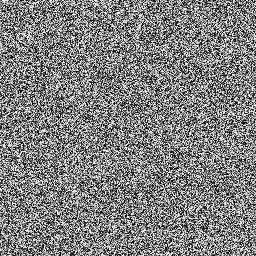
\includegraphics[width=\textwidth]{../images/snowfall.png}
            \subcaption{An image with no nearby pixel similarity, such as this image made up of random numbers, is assumed to never occur among real-world images.}
            \label{fig:snowfall}
        \end{minipage}
        \hspace{0.5cm}
        \begin{minipage}[b]{0.45\linewidth}
            \centering
            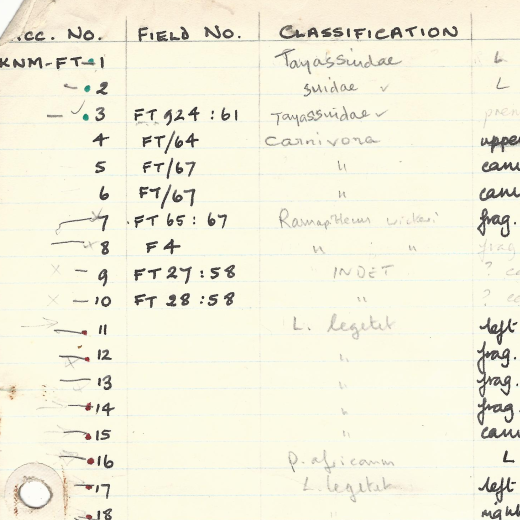
\includegraphics[width=\textwidth]{../images/cataloguesample.png}
            \subcaption{In a real image, most pixel colors are almost equal to neighboring pixel values. Segment from 
            the Fort Tenan Catalogue of the National Museum of Kenya.}
            \label{fig:snowfall2}
        \end{minipage}
    }

        \vspace{0.5cm}

    \resizebox{0.6\linewidth}{!}{%
        \begin{minipage}[b]{0.45\linewidth}
            \centering
            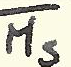
\includegraphics[width=\textwidth]{../images/molar.png}
            \subcaption{Transform invariance: the original tooth notation sample...}
            \label{fig:snowfall3}
        \end{minipage}
        \hspace{0.5cm}
        \begin{minipage}[b]{0.45\linewidth}
            \centering
            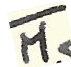
\includegraphics[width=\textwidth]{../images/rotated_molar.png}
            \subcaption{... still keeps its meaning of lower third molar after a transform}
            \label{fig:snowfall4}
        \end{minipage}
    }

    \caption{Visualization of the similarity and transform invariance assumptions encoded in the convolutional layer computation.}
    \label{fig:conv_assumptions}
\end{figure}

%the basic convolution
% convolution (cross-correlation)
% you have input and kernel. input: image matrix (2d) kernel: 2n+1 sized matrix (uneven to make it center around the input pixel processed)
% kernel slides like a sliding window through the input. for each middle position of the kernel:
% result is the dot product of the pixels in equal positions, eq 10.6
% if the image is rgb, kernel is 3d with depth 3. (bike fig 10.10 here)
The layer output computation on a convolutional layer is similar to the fully connected layer computation
presented in Equation \ref{eq:fc_layer}, but takes as input only a small region around each pixel instead of 
the whole input, and uses same weight parameters on all input positions. To achieve this, the weights of the 
layer only consist of a kernel, a small 
matrix of weights with uneven-numbered size in both the width and height dimensions \cite{princebook}. During the computation, the kernel 
acts as a sliding window, moving through every possible position on the input image. For each kernel position, an output 
value is produced by computing the dot product between the kernel and the kernel-sized input region around the processed position, and as usual, a bias term is added and the result is passed through the nonlinear activation function.
An example of this basic convolution operation on a grayscale image with kernel size 3x3 is given in Equation \ref{eq:convolution}. 
For a colored image with three color channels, the kernel becomes three-dimensional. An illustration 
of such case is found in Figure \ref{image:3dkernel}.

\begin{align}
    h_{ij} = a \left[ \beta + \sum_{m=1}^{3} \sum_{n=1}^{3} \omega_{mn} x_{i+m-2, j+n-2} \right],
    \label{eq:convolution}
\end{align}

\begin{figure}[h]
    \centering
    \includegraphics*[scale=0.4]{../images/3dkernel.png}
    \caption{An illustration of a convolution computation in the case of a color image, from \cite{princebook}.}
    \label{image:3dkernel}
\end{figure}

% % variants of the convolution: design decisions
% aspects: borders, channels, convolution size, dilation and stride
% default variant reduces size because border pixels cannot be used
% to combat that:
% zero or reflective, padding to keep output and input sizes equal, or valid convolution: dont compute positions where there are not enough previous inputs to use the whole kernel
% channels: run many convolutions in parallel -> more convolution kernel weights to learn
% size stride and dilation, figure 10.3
% size = kernel size
% stride = step between kernel computation
% dilation = kernel is interleaved with zeros, large region but less weights
% stride dilation size fig here
In implementing a convolutional layer, a few design decisions need to be made: how to handle border 
pixels, choosing a channel count, and the shape of the convolution kernel \cite{princebook}.
For the bordering pixels, where some kernel pixels fall outside of the 
input matrix, the options are to skip these computations, pad the input with zeros, or to pad the input 
by mirroring bordering pixels, the main difference of these being that not padding the input creates a 
result smaller than the input matrix. For the channel count, it has been found that sometimes 
running multiple convolutions side by side creates better results, and the optimal choice of channel count is 
application-dependent. The resulting channels are much like the familiar red, green and blue in an image, but do not 
have any human-decipherable meaning. Lastly, considering the kernel, three aspects need to be chosen: size, stride and dilation.
Size refers to, intuitively, the height and width of the kernel. The stride, commonly 1, controls by how many pixels the 
kernel is slid forward after each activation computation shown in Equation \ref{eq:convolution}. With dilation, the kernel itself 
is sparse: the weights are interleaved with a desired count of zeros. This allows for larger kernels without increasing parameter counts \cite{princebook}.

% % pooling
% usually conv layer followed by pooling layer
% pooling
% usually networks are constructed so that  layer by layer layer width decreases and has more depth (more channels, like red green and blue but not with this meaning)
% changing size more than by the few pixels present at image edges: max pooling. take maximum of 2x2 area, collect these values as the output activations. other, less popular variants: mean and average pooling
Usually, a convolutional layer is followed by a pooling layer. The pooling layer adds more nonlinearity to the network, 
and allows halving the layer size. The most common operation is the max pooling operation, where each output pixel is the maximum of
a 2x2 are in the input. Other, less popular operations include the mean and average pooling operations, where the output naturally 
is the mean and average of the small area, respectively. These operations allow for the common structure of convolutional networks, 
where the layer width and height progressively decrease as the computation proceeds \cite{princebook}.

% relevant here: present the ImageNet competition that has initiated many new architectures.
% % history bit: imageNet breakthrough models alexnet, googlelenet, vgg
% the what models. most influential
% historical scetch: alexnet \cite{alexnet} brought this to mainstream in 2012, imagenet 2014 saw GoogleLeNet \cite{googlelenet} and VGG \cite{vgg}.
% these highlighted because the architectures are utilized in handwritten character classification.
Many advances in convolutional networks have been motivated by the ImageNet image classification competition \cite{imagenet},
 that ranks models by their capacity of classifying images retrieved from the web to 1,000 distinct classes.
 The results are presented as top-1 and top-5 error rates, the percentage of samples 
where the correct class is not among the one or five most likely classes according to the network. Convolutional architectures
that have performed well in the competition have been found valuable in handwritten character classification, thus the 
breakthrough models presented next are experimented with in later parts of this work.
These most influential convolutional models in the history of the ImageNet challenge,  that
only rely on the basic convolution operation, are AlexNet \cite{alexnet}, 
the VGG model family \cite{vgg}, and
the Inception architecture used in GoogLeNet \cite{googlelenet}.

% alexnet, top5 error: 17\% best so far
% whats new regularization with dropout, large model, large conv kernels (11x11-3x3 kernels), 
% relu instead of previously popular tanhs sped up training, multiple GPUs used when training,
% normalization of convolution results, overlapping pooling (areas of pooling for each pixel overlap)
% impact: brought deep learning to center of ml research, deep nets seem to outperform humans in feature engineering.
The AlexNet convolutional neural network is perhaps the most influential deep learning model of all time, 
popularizing deep learning as a superior feature extractor compared to human-performed feature engineering (ref?).
% what was different
The breakthrough was achieved mainly by speeding up the training process by utilizing graphical processing units (GPU)
in training, a novel idea at the time, and simplifying the feed forward computation by replacing the previously popular 
hyperbolic tangent activation with the ReLU function (Equation~\ref{eq:relu}) \cite{alexnet}.
 This allowed training a larger, deeper network
with convolutional kernels up to the size 11x11, leading to nearly halving the best top-5 error rate with the score of
17,0\%. Other, more minor but still highly influential innovations were the normalization of convolution results, 
overlap in the pooling areas, and using dropout regularization, intruduced in Section~\ref{sect:heuristics}.

% googlelenet \cite{googlelenet} won 2014 with top 5 error rate  6,75\%.
% method: fixed number of allowed multiple-adds in forward pass, 
% used inception (named after we need to go deeper meme) layer: 1x1 3x3 and 5x5 s, also 
% sparse fully connected layers ie not all weights are connected.
% dimension reduction with 1x1 kernels
% to save compute. Also inspired by biological visual systems. allowed
% for deeper and wider network, turned out to be great in imagenet and 
% object detection.
The ImageNet competition of 2014 saw the next breakthrough innovation with the winning architecture of the GoogLeNet,
introducing the idea that smaller convolutional kernels with highly optimized training computation allows deeper,
and therefore more capable networks \cite{googlelenet}. The layer architecture, named Inception after the 'We 
need to go deeper' internet meme (see Figure~\ref{image:meme}), only used kernels of size 3x3 and 5x5, and
employed dimension reduction with 1x1 convolutional kernels. They also introduced sparsity by omitting connections on 
dense layers inspired by knowledge on the structure of biological visual systems. While these ideas were motivated
by performance-related reasons, the main aim of the study being to fix multiple-add operations available for training 
and to reach as high accuracy as possible, the resulting model ended up reaching a new best top-5\% error rate of 6,75\%
in ImageNet classification.
% sitten spesifiä. 3x3, 5x5 kernels only 1x1 kernels usage in dimension reduction, sparse dense layers to imitate human visual system

% vgg \cite{vgg}. achieved 6,8\% with imagenet 2014 postsubmission, submitted 7,3\% thus 
% second in competition. method: simple 3x3 convolutions, tested different depths. best depth 19.
% new that previous best models did big kernels and shallower nets. also good model because of 
% the simplicity + the paper included in appendix that demonstrated vgg as a feature extractor to 
% be used in transfer learning.
A close runner-up in the 2014 competition, the VGG model family again proved that deep networks 
with smaller kernels tend to outperform shallow, larger-kernel approaches \cite{vgg}. The approach 
of the experiments was to fix all kernels to 3x3 size, and to benchmark classification accuracy between 
different model depths. The deepest model with 19 layers was found to be most accurate, and additionally 
to be highly competitive as a feature extractor: an appendix of experiments reached new-best results on a variety of 
further classification tasks. While the 
best top-5 accuracy of 7,3\% ended up with a second place in the ImageNet 2014 competition, the  structural simplicity
and diverse learning capacity of the VGG models had a major influence on later deep learning research.

The architectures of the AlexNet, GoogLeNet and VGG models are summarized in Figure \ref{image:famouscnns}.

\begin{figure}[h]
    \centering
    \includegraphics*[scale=0.2]{../images/ebd.png}
    \caption{The meme that inspired the Inception architecture in GoogLeNet~\cite{googlelenet}, from~\cite{we_need_to_go_deeper}.}
    \label{image:meme}
\end{figure}

\begin{figure}[h]
    \centering
    \includegraphics*[scale=0.6]{../images/famouscnns.png}
    \caption{Architectures of AlexNet~\cite{alexnet}, GoogLeNet~\cite{googlelenet}, and VGG-16~\cite{vgg}, the 
    VGG model variant with 16 layers, from~\cite{zhangImagebasedMethodsDietary2023}.}
    \label{image:famouscnns}
\end{figure}

\subsubsection{Transformers and the multi-head self-attention}

\subsubsection{Autoencoders}

\subsection{Techniques and heuristics for improving performance}
\label{sect:heuristics}

\subsection{Transfer learning}

% % introduction
% relation to the coarse level training loop: how to initialize model parameters
% this sect from \cite{transferlearning_survey}. they initially formalized the problem and uniformized 
% the terminology

% % why transfer learning
% basics: what it is, basic premise: if you start out from a parameter configuration that solves a related 
% task well, there is lesser need to train to solve the new problem \cite{transferlearning_survey}.
% why: save compute (imagenet models vgg lenet alexnet training times 5 days to 3 weeks even when using GPUs \cite{vgg}) and data labeling (usual constraints in ml model building \cite{engbook})
% also why: training many parameters on a dataset overfits model to the dataset, so freezing layers prevents overfitting \cite{googlelenet},
% optimization idea: using pretraining that makes sense, you start from a parameter configuration in a 'basin of attraction'
% of a good minimum \cite{erhanWhyDoesUnsupervised2010}, ie a place where gradients point toward a good local minimum
%     training is strongly influenced by early examples so pretraining prevents overfitting to the supervised task 
%     get sgd trapped in a parameter space that is better so resulst is better even when target data is abundant \cite{erhanWhyDoesUnsupervised2010}    

% % types of transfer learning
% inductive transfer, transductive transfer, instance transfer, relational knowledge transfer
% task (inductive) transfer: tasks differ, data same or different
% task transfer relatedness + the more related the better results
%     negative transfer ie things made worse if things differ too much.
%     super important to consider the distance of transfer ie how similar the tasks are
% broad methods for inductive transfer: feature representation transfer, parameter transfer; priors or hyperparameters of model are assumed to be shared,
% instance transfer: reuse source data
% domain (transductive) transfer (only data differs)
% central idea in all of these: model first n-1 layers is a feature extractor
% seeing model as model doing the feature engineering: all but last layer are like 
% feature extraction that allows a linear model to be fit from features to output.
%     first layers learn lower level features, higher up more high level \cite{erhanWhyDoesUnsupervised2010}, so how much to freeze is about how
%     high level features are usable     
% relational-knowledge-transfer: when data is not i.i.d (not considered here)

% % using the terminology from  transfer learning, define my problem
% my task. source task is image classification with different data than mine
% inductive transfer where data and task differ.
% i will test both only feature representation transfer (re-search for optimal hyperparameters)
% and parameter transfer (use hyperparameters used in source model training)
% different countries mark tooth fossil in different notation, so fine-tune to adjust

% % how transfer learning is used in this work: skip anything that does not do transfer learning
% basically nowadays it is usually insensible to ever train from scratch \cite{cs231n_transfer_learning}
% therefore this work definitely transfer learns. also previous work that does not transfer learn is dismissed, 
% as it does not inform this case where target data is scarce

% \subsubsection{Foundation models}

% % - generalist models
% % 	- large unsupervised training data sets

% % why
% Idea: since transfer learning source task performance is not important, target task is the main point \cite{transferlearning_survey}, 
% you can come up with some nonsensical task such as map image to the same image to get unsupervised task, train 
% massively on massive compute, and use the model for varieties of tasks. idea: do as little as possible in the target domain
% because labeling is the expensive thing \cite{engbook}, this helps because unsupervised or selfsupervised allows 
% however many labeled samples one wants.

% % what
% come up with task with no value in itself but learns useful features. eg identity mapping in autoencoders,
% mask a part of an image and fill it in, get in a pair of images and say whether they are a transformation of one another.
% save the pretrained model, can be used with transfer learning in manymany tasks
% \cite{erhanWhyDoesUnsupervised2010}: why unsupervised pretraining works so well
% analytical analysis: seems to act as a regularizer
% generalization is better: intuition, model has seen a much larger variety of data 

% % ocr
% well this is used in ocr as well.
% so you would take some model trained on a large mass of data and then fine tune it on the characters

\section{Related work}

% intro
% this chapter presents related work from two angles
% angle 1: neural nets & transfer learning on similar problems
% angle 2: solutions to digitization of historical documents

This chapter presents related work from two viewpoints. First, in Section~\ref{sect:related_same_problem},
work on digitizing handwritten fossil catalogues is reviewed. As the work 
in this area is highly limited, Section~\ref{sect:same_solution} presents work using similar techniques 
to ones used here: publications aiming to recognize individual handwritten characters 
with deep neural networks and transfer learning with limited target domain data are presented.

% Search strategy: few seed papers and snowball search. Related conferences: 
% Frontiers in Handwriting Recognition

The literature search was conducted with a snowball search, proceeding with relevant forward and backward citations 
of a few key articles. Additionally, approximately last five to ten years of conference proceedings most relevant for this problem area were 
scanned. For related work on fossil digitization, any found work touching on the subject area will be commented on due to their 
limited amount. For work conducting a similar analysis of handwritten character recognition, more strict conditions were placed. 
For results, to be considered, the work had to be explicit about the best accuracy score achieved,
mentioning the size of the training dataset, number of characters within the classification problem, and the percentage 
of correct inferences with the test set. The source of the base model had to be given along with its source task, training data
and network architecture. The exact method of conducting the model fine-tuning had to be explicit enough to be reproducable,
work simply stating they used transfer learning or leaving gaps in the training process were omitted. Additionally, 
publication venue reputation and acceptable text and presentation quality were taken into account, and some work had to be
omitted because of undecipherable method descriptions or a lack of necessary detail.

% lists best accuracy clearly (percent, which dataset, number of classes)
% specifies the base model used (architecture and source domain dataset)
% specifies how transfer learning was conducted (not just used transfer learning)
% then reputable venue and acceptable quality of text and presentation,
%super subpar text was a frequent reason to skip a paper, they also often lacked relevant details

\subsection{Approaches to digitization of handwritten fossil catalogues}
\label{sect:related_same_problem}

% opening: the obvious solution: sit down and type is pretty much what is done now
While digitizing handwritten fossil catalogues holds,
should all state of the art optical character recognition and data management methods 
be in full use for solving the problem, perhaps a dramatic potential for improving 
the quality of paleoecological research, surprisingly little has as of now been done in this area.
Likely due to the simple fact that the problem has attracted little attention, 
most current work assumes the most rudimentary method: a human 
being sitting down, and transcribing.

% \cite{uhenCardCatalogsComputers2013} reviews various digital paleo data portals. encourages further digitization but 
% does not really mention how one should go about doing that
% \cite{mallisonDigitizingMethodsPaleontology2011} review of digitizing fossil data. only considers digitizing 
% physical bone pieces to various 3d images. does not take any stand on digitizing handwritten notes on the samples 
Due to large amounts of transcription work already done, digital repositories of fossil data do exist. A notable review 
by Uhen et al. \cite{uhenCardCatalogsComputers2013} reviews such databases and encourages further 
digitization of unpublished data, but does not take a stand on how one should complete such work.
Another more extensive review, a whole chapter on digitization methods in paleontology has been written \cite{mallisonDigitizingMethodsPaleontology2011},
but the chapter exclusively considers digitizing physical bone and plant pieces with various 3D imaging methods, and briefly touches on preferring digital journals over 
paper-printed distribution of research.

% \cite{groomImprovedStandardizationTranscribed2019} does identify my problem here: most fossil data is in handwritten paper 
% format with many things already known such as taxon. gives suggestions on data format and management but mostly assuming 
% that there is a human transcriber. presents ocr reading as a possibly one day possible option. Notes that especially cleaning of automated ocr read data is a hard problem.
For actual, automated handwriting recognition, a few mentions do exist in previous work. The data management themed 
article by Groom et al. \cite{groomImprovedStandardizationTranscribed2019} does identify the primary 
problem of this thesis: the article mentions the fact that most fossil data exists as handwritten records with sufficient information 
to conduct analysis without the physical sample, and a big advancement in data availability would be to efficiently and in a consistent 
manner convert this data to a structured database. Optical character recognition is presented, but more as a futuristic option 
not feasible with current methods, and any data quality suggestions implicitly assume that transcription is completed 
by a human being. This review is still relevant for automated digitization as many important considerations in data structuring,
standardization and quality management are presented - revealing the new challenge that should large-scale automated digitization succeed,
the next big line of work would be how to structure and manage the digital paleontological data.

% only work doing the exact same thing: \cite{shanmugavelHandwrittenOpticalCharacter2018}, but quality of the work is very poor, only 
% presents rudimentary very basic general aspects of image processing such as canny edge detection or contour detection from characters, 
% which is very very far away from working ocr. the paper lists absolutely no results but is an evidence that someone has somewhere at least 
% attempted this.
The only found work solving the exact same challenge as this work is thearticle by Shanmugavel et al. \cite{shanmugavelHandwrittenOpticalCharacter2018}.
While the problem is exactly the same, the methods only contain some of the most basic computer 
vision processes, edge and contour detection, and a complete lack of results reveal that not much was achieved in 
this project. However, it serves as a proof that such attempts have taken place in previous years.

% So: to the best of my knowledge there is no other work successfully reading handwritten fossil scans or cleaning 
% already automatically read systems outside of 2024 spring data science project for KNM, for which this is the 
% continuation. therefore also here i will do the simplest things first, since it is a good idea to start with simple and 
% once successful, proceed to harder problems that would digitize and clean more data.
Concluding the review on research articles about digitizing handwritten fossil data, it seems that no successful projects
have as of yet been completed outside of the Data Science student project in spring 2024 for the National 
Museum of Kenya, for which this work is a continuation. For this reason, the experiments in this thesis will 
start out with the simplest problem reductions and only present more advanced techniques as ideas for future work.
The rationale behind this decision is that since not much has yet been done, it is best to start out from 
simple and established implementations to verify simple hypotheses before proceeding to more recently developed mehods.

\subsection{Approaches to handwritten character recognition with small target domain datasets}
\label{sect:same_solution}

Found papers:

\cite{akhlaghiFarsiHandwrittenPhone2020} \cite{chatterjeeBengaliHandwrittenCharacter2020} \cite{thuonImprovingIsolatedGlyph2022}
\cite{goelHandwrittenGujaratiNumerals2023} \cite{goelPreTrainedCNNBased2022} \cite{limbachiyaIdentificationHandwrittenGujarati2022}
\cite{rasheedHandwrittenUrduCharacters2022} \cite{rizkyTextRecognitionImages2023} \cite{shoponBanglaHandwrittenDigit2016}
\cite{zunairUnconventionalWisdomNew2018} \cite{zhaoIncrementalRecognitionMultiStyle2024}

\section{Experimental setup}

\subsection{Data description}

\subsubsection{Notes on creating the dataset}

\includegraphics*[scale=0.2]{../images/superambiguous_data_sample.png}

\subsubsection{Unicode characters used for data labeling}

%tricks to label to make model work easier
To label the text found in cropped-out tooth fragment handwriting images, a few nonobvious 
conventions had to be set in place to construct a labeling system that can be assumed to 
be easier to learn for a machine learning model. The main guiding rule in these decisions was 
to encode each feature in the text in one consistent manner. What is meant by features and manners 
of denoting is explained next.

%\cite{unicode_homepage}
%expain unicode: graphene & code point 
%    explain: unicode has graphenes with code points. eg a is one graphene one code point,
%    à is one graphene two code points (dot on top and the letter). the top thing -like characters will be called 
%    "modifiers".
%general aim: one concept, one code point -> model able to figure out the connection between image and concept 
%concept: "number 2" "a character with a line on top"
%Also on the other hand using one modifier for all lowercase characters allows 
%the model to understand that there is a similarity between all lowercase characters.
%The intention is that one idea about a character is encoded as one code point, so that 
%the model can learn the mapping from the image of the character to the code point 
%combination
The unicode system \cite{unicode_homepage} constructs all known characters as signs called graphenes.
Each graphene can consist of any number of code points, with each code point having an unique identifier, denoted with "U+code point id".
Examples of graphenes with one code point are latin letters, such as 'K', special characters, such as '@', '\%' and '+',
or letters from different writing systems, such as '$\omega$', '$\aleph$' or '$\mathfrak{A}$'.
 Examples of multi-code point graphenes 
are latin letters with accents, such as '$\hat{\text{e}}$', or emoji characters with non-default skin tone, such as {\twemoji{thumbs up: dark skin tone}}.
Code points added to the main code point, such as the circumflex accent '\^ ' are called modifiers.

The guiding principle in labeling the data was to encode each concept in the text as one unicode code point. A concept could be, for 
instance, the number two, or a character being positioned in subscript. The aim of this decision is to allow the model 
to find common image traits between characters of a similar type: a subscript character has dark pixels in lower positions, and shapes of all 
number two's have similar curvatures, for instance. As a second principle, it was chosen that each single character in the image, such as "letter C" 
or "a subscript four with a horizontal top line", would always be labeled as one graphene. 
These rules makes the encoding choices nonobvious: for example, 
a subscript number two would intuitively be labeled as the unicode code point '$_2$', but this was not done, 
since this graphene does not contain the code point for number two, 
and as a one code point graphene has no code point to extract to be used among the other subscript numbers.
Another intuitive choice, '\_2', would violate the one graphene per character rule.

%data characters:
%markings contain letters and numbers with no line, line on top or line at the bottom.
%Each character can be lower- or upper script.
%insert here example img of characters
The special characters in the dental fossil handwriting consist of sub- and superscript numbers, and characters with a horizontal line on 
top or bottom. Additionally, these two modifiers sometimes co-occur. Both denote which jaw the fragment is from: 
subscript and horizontal line on top of the character denote lower jaw, whereas superscript or line at the bottom of character 
signal upper jaw. In a few rare occurences, fractions are present 
to denote which proportion of the tooth is remaining in the sample. 
Note that ambiguous notations of for instance subscript number with a horizontal line at the bottom are allowed with this writing system.
The labeling notation chosen preserves the option to label these ambiguities.

%The modifiers used for these: 
%macron with lower ($\bar{\mathrm{A}}$) and upper variant.
%super/subscript: lower and upper script character set is incomplete for this purpose (eg 3 with upper macron and lower script needed)
%- from the model perspective 3 and $_3$ are no more similar than A and B, however, 
% therefore:  Therefore, modifier was used.
% there is no lower or upper case modifiers in unicode
%the caron ($\check{\mathrm{A}}$) was chosen as the lower script modifier, and the circumflex accent ($\hat{\mathrm{A}}$)
%as upper script. These were chosen since the arrow-like modifier pointing up or down
%is maybe the most logical placeholder for the missing modifier. More traditional 
%workarounds of missing upper or lower script, the underscore "\_" and separate 
%caret character "\^ " were not used because they would violate the one graphene one character rule

The following code points were chosen to denote the tooth marking system in the data labels.
The base code point modified with unicode modifiers was always chosen to be the latin letter or number present in the character. In the case of 
fractions, the number in the denominator was chosen as the base code point. The horizontal line on top of a character was denoted with the
combining macron modifier (U+0304, eg. $\bar{\text{A}}$), the line at the bottom respectively with the combining macron below (U+0331, eg. \underline{A}).
As the unicode system lacks sub- or superscript modifiers, other accent modifiers were used instead. A subscript character was denoted with the combining caron (U+030C, eg. $\check{\mathrm{A}}$), and respectively the superscript with the combining
circumflex accent (U+0302, eg. $\hat{\text{A}}$). For fraction nominators, a modifier was chosen for each digit present in the dataset (TODO: add here after chosen).
These choices were made to improve human readability of the dataset, as the modifier choices are not relevant from the model perspective. A sample of the handlabeled 
dataset can be found in Figure~\ref{table:input_images}.

\begin{table}[h!]
    \centering
    \begin{tabular}{|c|c|}
        \hline
        \textbf{Input Image} & \textbf{Label} \\
        \hline
        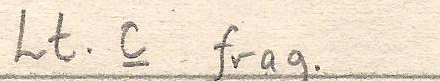
\includegraphics[width=0.3\textwidth]{../images/data_samples/canine.png} & Lt. \underline{C} frag. \\
        \hline
        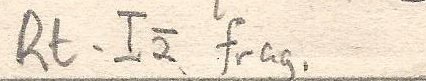
\includegraphics[width=0.3\textwidth]{../images/data_samples/lowjawincisor.png} & Rt. I$\bar{\check{2}}$ frag. \\
        \hline
        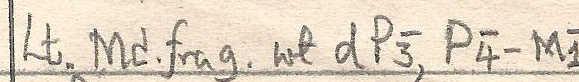
\includegraphics[width=0.3\textwidth]{../images/data_samples/multipleteeth.png} & Lt. Md. frag. wt dP$\check{\bar{3}}$, P$\check{\bar{4}}$-M$\check{\bar{1}}$\\
        \hline
        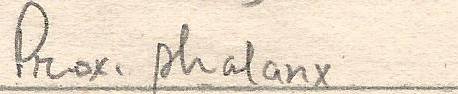
\includegraphics[width=0.3\textwidth]{../images/data_samples/nontooth.png} & Prox. phalanx \\
        \hline
        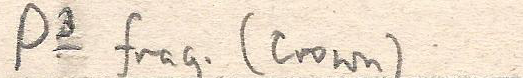
\includegraphics[width=0.3\textwidth]{../images/data_samples/smudged.png} & P$\hat{\underline{\text{3}}}$ frag. (Crown) \\
        \hline
        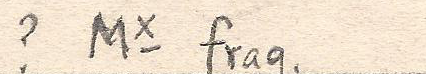
\includegraphics[width=0.3\textwidth]{../images/data_samples/underlinedx.png} & ? M$\hat{\underline{\text{x}}}$ frag. \\
        \hline
    \end{tabular}
    \caption{Samples of input images and their corresponding labels.}
    \label{table:input_images}
\end{table}


\subsection{Data preprocessing}

\subsection{Methods: base models and transfer learning tehniques}

\subsubsection{Problem formulation}

\subsubsection{Base model selection}

\subsubsection{Transfer learning method selection}

\section{Results and discussion}

\section{Conclusions}

% why word bounding box worked badly and how it could be improved
% how this could be continued
% main problem in working with azure bounding boxes: incorrect identification of word bounding boxes.
% encoding prior knowledge should work better: M1-3 is a word for instance, azure did stuff like m, 1-, 3
While this work managed to accurately clean a part of dental markings present in the catalogues, 
there are several potential directions to significantly improve the digitization of such catalogues in general, the main direction 
being improving the quality of word-location defining bounding boxes. The main problem in the bounding boxes provided 
by Azure Vision~\cite{azurevision} was that the dental marking words were often cut across many words or were present 
as a part of a longer word. This is likely due to the space width varying greatly between different pieces of 
handwriting. To improve the correctness of handwriting segmentation to words, developing a fine-tuned word detector 
could improve the result: a specialist model encoded with knowledge on what kinds of words are more likely to be 
present in the data would likely be much better at finding correct bounding boxes. An example of 
such case is seen in Figure~\ref{image:hardsentence}: a segmenter with the knowledge of tooth marking notation could 
easily see that the $\text{dm}_{3-4}$ section is one word, which is difficult to a generalist model 
due to the spacing between the characters.

% point of this paragraph: object detection is a harder task and has gotten attention from cv research in recent years.
% on hardness. from computer vision lecture 11 \cite{ruotsalainen2024}
% object bounding box detection requires higher resolution images and ground truth labels -> labeling effort is 
% big, compute needed. one idea is to take premade bounding boxes by generalist ocr word detectors and for example
% infer they are correct by matching with a vocabulary of known correct words to exist in fossil catalogues.
% pointers to research work on computer vision object detection
% on recent work. several new advances seem without testing promising, but unfortunately their main problem is differnet from ours so not directly applicable
%I quickly tested a state of the art object detection model the yolo10, variant of popular object detector yolo\cite{redmonYouOnlyLook2016}
%  untuned, on huggingface api, the yolo10 \cite{OmouredYOLOv10DocumentLayoutAnalysisHugging2023}. The performance 
% was poor, see fig, probably since object detection usually does 3d object detection in a 3d scene, so one should either 
% fine tune or find a ocr bounding box detector. then there is open-vocabulary object detector which you can tell what objects 
% are present \cite{YOLOWorldRealTimeOpenVocabulary}. we could just say there are teeth and words. 
% then also a very recent publication on detecting text on images \cite{longHierarchicalTextSpotter2024}.
% benefit of these is that they are fine-tunable which the commercial azure api is not. 
% then also detectron \cite{Detectron} from meta for object detection
% one could also run more sophisticated 
% tooth or not classification on azure output, which could work very well but relying on a paid service is not ideal 
% for open access solutions.
The problem of finding objects in images is much harder than image classification and has attracted attention 
from the computer vision research community very recently. 
Main reasons for the difficulty are the labour required to obtain ground truth bounding boxes and 
the fact that object detection requires better image resolution to work well, therefore requiring more computational resources \cite{ruotsalainen2024}.
One way to circumvent manual annotation for fossil catalogues could be to automatically detect correct bounding boxes 
from commercial OCR engine output files for instance by regular expression matching the word readings with a vocabulary of words likely to be 
present in fossil catalogues, much like the approach implemented in this work.
For the detection model, several recent advances seem promising, but might not be directly applicable without fine-tuning 
due to the fact that the standard problem of object detection is to detect three-dimensional objects in 3D scenes, which is 
quite different from word detection on a flat, scanned document. This is likely the reason why an initial experiment 
ran on the Hugging Face API version~\cite{OmouredYOLOv10DocumentLayoutAnalysisHugging2023} of YOLO-10~\cite{wang2024yolov10}, a variant of the highly influential object detector YOLO~\cite{redmonYouOnlyLook2016},
resulted in a very poor segmentation found in Figure~\ref{image:yolo}: the entire image was segmented as one object.
Some possibly more applicable models, however not as easily testable due to lesser popularity, 
are the open-vocabulary version of YOLO~\cite{YOLOWorldRealTimeOpenVocabulary},
 the hierachical text spotter~\cite{longHierarchicalTextSpotter2024}, and the Detectron by Meta~\cite{Detectron}.
 However, due to the catalogue-specific problem illustrated in Figure~\ref{image:hardsentence}, it is likely that these 
 models would require well-optimized fine-tuning to work well. Experimenting with such implementations is a 
 substantial effort and was omitted from this work to keep the scope reasonable.

% % improving MPI/upperlower classification (not as hard so not as relevant perhaps)
% ways to improve the result of image classification obtained here 
% test svm after feature extraction instead of the dense layers + softmax. My most recent model was from (insert year),
% since then imagenet classification has advanced, so try using a newer base model. these can be harder to obtain 
% since they are not as established, I could just fetch models from torchvision.models, newer ones are not present there.
% with a good object detector probably we can get to more variaty of tooth marking images (maybe a fig of examples?)
% so the classification task would become more complicated. Still, the downstream tooth marking image to tooth task 
% is a relatively easy classification problem comparing to eg imagenet, so the main challenge is definitely finding words and
% classifying them to tooth or not.
Another possible line of extending the work would be improving the accuracy of the image classification to tooth type. 
Some ideas are to use a support vector classifier instead of fully connected layers combined with the softmax activation 
on the last layer, and to experiment with more recent ImageNet classifiers with better top-5 and top-1 error rates.
However, using the newer models would require more effort since good pretrained weights are 
more difficult to find for the less established models, and there is less evidence of their applicability to downstream tasks.
Improving the model would still be highly useful, since a more sophisticated word object recognizer would result in a more 
variable set of tooth marking images to be given to the tooth type classifier, making its classifying problem much more difficult. 
Still, the object detection problem should be given more attention since even the 
potential harder variants the dental marking classification task are relatively simple image classification problems when comparing 
them to challenges such as basic ImageNet classification.

\begin{figure}[h]
    \centering
    \includegraphics*[scale=0.3]{../images/yoloresult.png}
    \caption{Preliminary object detection test with the YOLO-10 object detector using the Hugging Face inference API~\cite{OmouredYOLOv10DocumentLayoutAnalysisHugging2023}.}
    \label{image:yolo}
\end{figure}

\begin{figure}[h]
    \centering
    \includegraphics*[scale=0.8]{../images/hardwordsegmentation.png}
    \caption{Example of a sentence hard to segment to words without context knowledge}
    \label{image:hardsentence}
\end{figure}

\printbibliography

\end{document}